\chapter{MongoDB}\label{mongodb-fabian}

\section{Einleitung}\label{einleitung}

\begin{figure}[h]
	\centering
	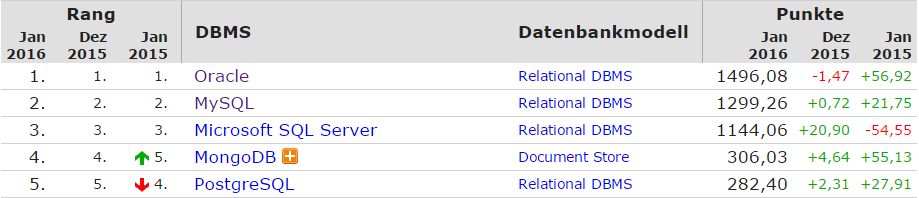
\includegraphics[width=0.7\linewidth]{figures/db-ranking.png}
	\caption{Datenbanken Ranking Datenquelle: db-engines \cite{db-engines:mongodb}}
	\label{f:mongodb:ranking}
\end{figure}

Die Entwicklung von MongoDB wurde im Jahr 2007 von dem Unternehmen 10gen
ins Leben gerufen. Als Programmiersprache wurde C++ verwendet.
Da die Datenmengen seit einigen Jahren durch Big Data immer rasanter steigen \cite{csc:bigdata}
werden die Skalierbarkeit und die Performanz bei großen Datenmengen zu
immer wichtigeren Themen. MongoDB wirbt mit Flexibilität, Skalierbarkeit und
Performanz. Dies soll durch denn Einsatz von verteilten Systemen
ermöglicht werden. Der Name mongo leitet sich aus dem Wort humongous ab,
welches gigantisch bedeutet. Hierdurch wird auf die Idee eine Datenbank
für große Datenmengen zu entwickeln angespielt.

Wie in der Abbildung \ref{f:mongodb:ranking} zu sehen steht MongoDB aktuell auf dem
vierten Platz der populärsten Datenbanken. Damit ist sie hinter drei
klassischen Relational Database Management System (RDBMS) die populärste
NoSQL-Datenbank. Bei der aktuellen Version handelt es sich um die 3.2.

\section{Konzepte}\label{konzepte}

\subsubsection{Grundlagen}
Eine herkömmliche RDBMS besteht aus Datenbanktabellen, die einem festen
Schema unterliegen. Bei MongoDB dagegen handelt es sich um eine
Schema-freie, dokumentenbasierte Open-Source-Datenbank. Diese beinhaltet
Sammlungen, die jeweils aus mehreren Dokumente ohne ein festes Schema
bestehen. Jedes Dokument darin kann sich von den Feldern und Strukturen
von den anderen unterscheiden. Dokumente bestehen aus mehreren
Schlüsselwert-Paaren und stellen die Basiseinheit für Daten dar.
Diese Daten werden im sogenannten BSON Format gespeichert und
ausgetauscht. Dabei handelt es sich um die binäre Variante von JSON.

\subsubsection{Datentypen}
Die hierbei verwendbaren Datentypen sind die bekannten Standard-Datentypen
Integer, Float, Boolean, String, Array. Zusätzlich gibt es noch die Date, Embedded-Doc, DBRef und
ObjectID.

\subsubsection{Referenzierung}
Es gibt unterschiedliche Wege in der Datenbank zu referenzieren.
Eine Möglichkeit ist die Referenzierung durch die Verschachtelung der Dokumente.
Hierbei referenziert ein Dokument auf ein anderes einzelnes Dokument.
Allerdings führt dies zu einer hohen Komplexität, wenn z.B. ein Update auf
eine verschachtelte Information durchgeführt werden soll.

Bei der ObjectID handelt es sich um die Standard ID, die jedes Dokument
aufweist. Diese wird bei der Erzeugung eines jeden Dokuments generiert
und ist durch ihren komplexen Aufbau eindeutig. Bei Verwendung der
ObjectID handelt es sich im Gegensatz zu verschachtelten Dokumenten um
einen ``echten'' Join. Hier referenzieren mehrere Dokumente auf ein Dokument
in der gleichen Collection.

Der DBRef entspricht dem Fremdschlüssel aus dem
RDBMS. Also dient er als Identifier für Dokument, Collection und
Datenbank. Dadurch können mehrere Dokumente auf ein Dokument in einer anderen
Collection referenzieren.

MongoDB verwendet eine integrierte Query Language. Durch
diese können Abfragen, Replikationen und Sharding auf den mongos ausgeführt werden.

\subsubsection{Replikation}
Die Replikationen spielen bei NoSQL-Datenbanken eine zentrale Rolle. Diese sorgen für die Synchronisierung von Daten über mehrere
Server. Im Gegensatz zu RDBMS sind bei NoSQL-Datenbanken Rundanzen erwünscht.
Denn diese dienen sowohl als Backup der Daten, als auch um die Performanz bei
Leseoperationen zu steigern. Nachteil hierbei ist, dass die Konsistenz nicht mehr gewährleistet werden kann.
Ein weiterer Nachteil ist das mehr Speicherplatz benötigt wird. Dies sollte jedoch, da es um
verteilte Systeme geht, kein Problem darstellen.

Bei MongoDB funktionieren die Replikationen nach dem Master-Slave-Prinzip. \cite{mongodb:replication}
D.h. es existieren in der Datenbank lauter Replikationssets. Diese bestehten
aus einer primären Replikationen und beliebig vielen sekundären Replikationen, also Kopien von den
primären Replikationen. Alle Schreiboperationen gehen nur an die primären Replikationen. Diese synchronisieren ihre sekundären
Replikationen erst nach und nach. Das bedeutet, dass die Daten für eine gewisse Zeit
inkonsistent sind. Es kann daher keine Konsistenz zum Transaktionszeitpunkt garantiert werden wie bei RDBMS.

Im schlimmsten Fall funktioniert eine Schreiboperation auf der ausführenden primären Replikation und
diese fällt aus bevor sie die Schreiboperation an die sekundären Replikationen
weitergegeben konnte. Dies führt nämlich zu Datenverlust, ohne das MongoDB
etwas davon mitbekommt. Die Datenbank denkt dann das die Operation
erfolgreich ausgeführt wurde, obwohl das gar nicht der Fall ist.

Jetzt könnte man sich fragen, warum eine Schreiboperation nur auf einer der primären Replikationen ausgeführt wird.
Dadurch wird ja ein Flaschenhals bei der Performanz von Schreiboperation erzeugt.
Das stimmt zwar, aber der Vorteil des automatischen failover überwiegt. Falls also
die primäre Replikation bei dem Versuch eine Schreiboperation auszuführen nicht erreicht werden kann,
wird eine der ehemals sekundären Replikationen zur neuen primären Replikation definiert. Da es sich bei den sekundären Replikationen
um eine Kopie der primären handelt ist dies ohne großen Aufwand möglich.

Für Leseoperationen kann man MongoDB nach seinen eigenen Wünschen konfigurieren. \cite{mongodb:replication}
Eine Möglichkeit ist die Last auch auf sekundäre Replikationen zu verteilen.
Vorteil hiervon wäre eine bessere Performanz bei Leseoperationen, da man quasi einen
Skalierungeseffekt erhält. Allerdings kann man nicht sicher
sein, dass alle sekundären Replikationen die aktuellsten Daten beinhalten.
D.h. man bekommt unter Umständen alte Datenstände zurück. Daher kann es durchaus sinnvoll sein
MongoDB so zu konfigurieren, dass auch Leseoperationen nur von der primären Replikation durchgeführt werden.

\subsubsection{Sharding}
Um den in der heutigen Zeit nicht ungewöhnlichen stark wachsenden Datenmengen
zu begegnen gibt es das automatische Sharding \cite{mongodb:sharding}. Dieses sorgt für die
Verteilung der Daten über mehrere Server. Dies wird auch als
horizontale Skalierung bezeichnet. Hierdurch ergeben sich vielfältige Vorteile. Zum
einen verursacht das vertikales Skalieren, also der Einsatz immer
besserer Hardware exponentielle Kosten und ist auch nicht unbegrenzt möglich. Zum anderen ist der lokale
Speicher möglicherweise einfach nicht groß genug. Da man durch das automatische Sharding einfach zusätzliche Server
in das Datenbank System integrieren kann hat man diese Probleme nicht.

Die Komponenten sind Shards, Config Server und mongos. Jedes Shard entspricht einem oben
beschriebenen Replikationsset. Die Config Server beinhalten die
Metadaten von dem Cluster. Sprich eine Map von den angefragten Daten und
ihren Speicherorten. Um eine ausreichende Redundanz und Verfügbarkeit gewährleisten zu können
muss es drei Config Server geben. Dann gibt es noch die mongos. Diese
werden von der Applikation angesprochen und führen die query Kommandos
aus.

Um Sharding durchführen zu können wird außerdem Map and Reduce eingesetzt. Map and Reduce entspricht dem Group Operator in RDBMS.
Hierbei werden auf allen Servern parallel Map Operationen ausgeführt. Danach fast die Reduce Operation alles zu einem Ergebnis zusammen.

\subsubsection{BASE}
Bedingt durch die oben genannten Konzepte ist eine strenge Einhaltung der ACID (atomar, consistency, isolation, durability) Kriterien nicht möglich. Es wird ein Tradeoff von Konsistenz und Isolation zu einer besseren Performanz und Skalierbarkeit eingegangen. Da man auf Konsistenz allerdings nicht vollständig verzichten kann wird das abgeschwächte BASE (Basically Available, Soft state, Eventual consistency) angestrebt. Hierbei wird nur eine "weiche" Konsistenz gewährleistet.

\section{Usecases}\label{usecases}

Ein großer Vorteil von MongoDB ist, dass es schnell einsetzbar / konfigurierbar ist.
Außerdem stellt eine sich öfter ändernde Datenstruktur kein Problem da.
Damit eignet sie sich hervorragend für rapid prototyping bei kleineren Projekten.

Allerdings eignet sie sich durch das Replizieren und ihre Skalierfähigkeit auch für große Datenmengen
und besonders für Leselastige Anwendungen.

Den Hauptnachteil stellt die nicht wirklich gegebene Konsistenz dar.
Dadurch steigt der Aufwand für die Anwendungsentwicklung, die daraus entstehende Probleme abfangen muss.

MongoDB wird damit für viele Anwendungsfälle nicht geeignet sein, da man einen Tradeoff eingehen muss.
Welche Datenbank verwendet werden sollte hängt somit immer von den konkreten Anforderungen ab.

\section{Mongoose}\label{mongoose}

Bei Mongoose handelt es sich um ein Modul für das NodeJS Framework.
Durch dieses Modul wird Object Data Modelling (ODM) im Zusammenhang mit MongoDB ermöglicht.

Der Hauptvorteil von Mongoose besteht in der Abstraktion von Daten der MongoDB.
Man kann sich Mongoose als abstrakte Schicht über MongoDB, der die schemalosen Daten auf Objekte mappt vorstellen.
Viele Entwickler, die es vorher mit SQL-Datenbanken zu tun hatten dürften damit wesentlich besser zurecht kommen,
als mit den dynamischen Sammlungen von MongoDB.

\begin{figure}[h]
	\centering
	\begin{lstlisting}
		var mongoose = require('mongoose');
		mongoose.connect('mongodb://localhost/test');

		var Cat = mongoose.model('Cat', { name: String });

		var kitty = new Cat({ name: 'Zildjian' });
		kitty.save(function (err) {
		if (err) // ...
		console.log('meow');
});
	\end{lstlisting}
	\caption[mongooseSchema]{Programmbeispiel \cite{mongoose:bsp}}
\end{figure}

Anhand dieses Beispiels erkennt man wie mithilfe von Schemas und Models Strukturen definiert werden.

Außerdem bietet diese Bibliothek auch noch einige andere Funktionalitäten. Unter anderem zum Einsatz von Middleware, Plug-Ins und zur Validierung.

Mongoose verwendet das Konzept Active Records. Dies ist ein durchaus umstrittenes Konzept,
da es auf der einen Seite als leicht und schnell erlernbar gesehen wird,
allerdings auf der anderen Seite das Testen erschwert und zu Flaschenhälsen in der Performanz führt. \cite{ormPattern:activeRecord}

Die Dokumentation auf der offiziellen Webseite ist sehr unübersichtlich. Hierdurch wird das Arbeiten mit dieser Bibliothek erschwert.

Die aktuelle Version von Mongoose wurde im Januar 2016 als 4.3.5. veröffentlicht.
